\documentclass[12pt]{article}

\usepackage{graphicx}
\usepackage{caption}
\usepackage{amsmath, amssymb, amsthm}
\usepackage{booktabs}
\usepackage{enumitem}
\usepackage{geometry}
\geometry{margin=1in}
\usepackage{xcolor}
\usepackage{float}
\usepackage{tabularx}
\usepackage[normalem]{ulem} % normalem keeps \emph working normally
\usepackage{algorithm}
\usepackage{algpseudocode}
\usepackage[colorlinks=true, allcolors=blue]{hyperref} % load near the end
\usepackage[capitalise]{cleveref} % must be loaded after hyperref

\title{NPSC3000 End of Year Report: Can Reinforcement Learning Outperform Traditional Methods for Cloud Resource Allocation}
\author{
\textbf{Student:} Ty Riekert \\
\textbf{Supervisor:} Elham Mardaneh \\
\textbf{Co-supervisor:} Tony Mathew
}
\date{October 2026}

\begin{document}
\maketitle

% =====================================================================
\begin{abstract}
Resource allocation (RA) is a critical problem for cloud providers \cite{saidi2023, sdn2021, vinothina2012, parikh2013, mohamaddiah2014}: a shared pool of physical servers must serve a continuous stream of user jobs while meeting deadlines and limiting energy use. Classical scheduling methods are known to struggle with the dynamic, multi-objective nature of this problem \cite{lbts2024, 10854610, DAHMANI2025100616}, while reinforcement learning (RL) has shown promise in similar settings \cite{saidi2023, autoscaling2023, lbts2024, dynamic2026}. This project asks \emph{under which objectives and conditions RL outperforms classical scheduling methods}. We model cloud RA as a multi-resource scheduling problem in two settings, offline (all jobs known in advance) and online (jobs arrive randomly), and formulate it as a Markov decision process. Six action-space designs were trained with proximal policy optimisation (PPO) and advantage actor-critic (A2C) under one uniform tuning and training protocol, and compared on 50 held-out instances against 49 dispatching heuristics and the CP-SAT exact solver. On the main objective, weighted squared tardiness, the best RL agent comes within 5\% of the best heuristic offline but does not beat it, and only ties the best heuristic when all jobs are equally important. Once linear tardiness or the number of late jobs is added to the objective, RL beats the best heuristic by 2--10\% offline. Online, RL needs far more training: with more steps the best design closed most of its gap to the best heuristic but did not overtake it. RL never beat the heuristics when energy was part of the objective. Overall, RL is most competitive when the objective combines several goals that no single hand-designed rule targets, and when jobs differ in importance.
\end{abstract}

\newpage
% =====================================================================
\section{Project Aims and Deliverables}
The aim of this project is to formulate cloud resource allocation as a mathematical optimisation and reinforcement learning problem, and to rigorously evaluate RL models against established methods. The specific deliverables are:
\begin{itemize}
    \item Conduct comprehensive research on current findings and machine learning in cloud resource allocation
    \item Formulate a mathematical model of the cloud RA problem, expressed as a resource-constrained scheduling optimisation problem
    \item Create a corresponding Markov Decision Process (MDP) formulation for the reinforcement learning agent
    \item Implement the code of the scheduling environment
    \item Implement the code for the reinforcement learning agent(s)
    \item Evaluate the trained agents against classical scheduling heuristics to determine under what conditions reinforcement learning outperforms traditional methods.
\end{itemize}
The last item is not a single `train and compare' run, but an iterative process repeated throughout the second half of the project: a constant loop of training, evaluating against baselines, investigating behaviour and faults, checking them against the literature, and revising.

% =====================================================================
\section{Background}
\subsection{Cloud Computing}
Cloud computing refers to the use of computing services and resources delivered over the internet, and resource allocation (RA) is one of the most critical challenges facing cloud providers today \cite{saidi2023, huawei2022}. As cloud infrastructure underpins the majority of modern computing services, effectively allocating physical resources, like compute or network bandwidth, to a continuously arriving stream of workloads has become of vital importance to providers \cite{sdn2021}. Poor allocation leads to poor response time, throughput, makespan, utilisation, energy efficiency and environmental sustainability \cite{cloudkpi2010, dvbpp2026, mohamaddiah2014, anuradha2014}.

\subsubsection{Cloud RA}
Cloud RA can be decomposed into several coupled problems. Virtual machine (VM) placement decides which physical server hosts each virtual machine, subject to the server's CPU, memory and other capacities, and is widely regarded as the core RA subproblem \cite{saidi2023}. Task scheduling decides when and on which resource each user task runs; depending on the setting it may prioritise execution time, response time, deadlines or an even spread of work \cite{lbts2024}. Autoscaling dynamically adjusts resource capacity to match fluctuating demand \cite{autoscaling2023}, and load balancing distributes incoming tasks evenly to avoid hotspots \cite{lb2024}. This project studies the task-scheduling view: deciding when and where each job runs.

Solutions to these problems generally fall into three categories:
\begin{itemize}
    \item \textbf{Exact methods.} Algorithms, such as integer and constraint programming, that are guaranteed to find an optimal solution given enough time.
    \item \textbf{Approximation methods.} Used when exact methods become computationally infeasible. \emph{Heuristics} are problem-specific rules, designed by people from domain knowledge, that quickly construct or improve a single solution (for example, ``always run the job with the earliest deadline''). \emph{Metaheuristics} are general-purpose search strategies, such as particle swarm optimisation, that guide heuristic methods through the space of solutions \cite{alkhalifa2025comparative}.
    \item \textbf{Machine learning (ML).} Methods that learn a decision rule from data or experience instead of having it written by hand. For scheduling, a model is trained on many example problems, and the trained model then makes allocation decisions on new problems.
\end{itemize}

Exact methods guarantee optimality, but scheduling problems of this kind are NP-hard \cite{lenstra1977complexity}, so their run time grows rapidly with problem size; in practice they are limited to small instances, or are stopped early and used for the best solution and bounds they have found. Heuristics and metaheuristics scale well but give approximate solutions with no guarantee of quality. Systematic reviews identify four recurring limitations of these approximation methods in cloud RA: scalability to large systems, adaptability to changing workloads, handling several conflicting objectives at once, and the need for real-time decisions \cite{mohamaddiah2014, lbts2024, 10854610, DAHMANI2025100616, ml_ra_litrev2025, hu2021attend2pack}.

\subsubsection{Motivations for Machine Learning}
These limitations motivate a growing body of work applying machine learning, and reinforcement learning specifically, to combinatorial and scheduling problems. A fixed heuristic relies on its designer's intuition about what makes a job important, and applies that rule unchanged in deployment. RL still requires design choices, such as what to optimise, but the rule for assigning jobs to machines is learnt during training, in an environment that should reflect the deployment environment \cite{ml_ra_litrev2025}. Systematic reviews of RL for scheduling and bin packing report encouraging growth in this area \cite{DAHMANI2025100616}, and prior systems such as DeepRM \cite{mao2016deeprm} and Decima \cite{mao2019decima} showed learned schedulers matching or exceeding hand-designed rules on cluster workloads.

This project examines two actor-critic RL methods, Proximal Policy Optimisation (PPO) and Advantage Actor-Critic (A2C), the synchronous version of A3C \cite{schulman2017ppo, mnih2016a3c, konda1999actorcritic, chadia2023understandingRL}. It also examines RL as a selection hyper-heuristic, where the agent chooses between dispatching rules \cite{burke2013hyperheuristicsurvey, lassoued2026hyperheuristic, cie2025dispatchruleselection}, and hybrid designs in which RL learns job priorities while a fixed rule places jobs on machines \cite{min2022atctuning, chen2024drlgphh}. These are compared against classical dispatching heuristics, a metaheuristic and an exact solver \cite{vepsalainen1987atc, ortools}.

\subsubsection{Project Motivation}
RL for cloud RA is an active research area \cite{ml_ra_litrev2025, DAHMANI2025100616}, but existing papers mostly optimise only a few objectives and compare against a limited set of baselines. Most model the problem as bin packing or VM placement, and many focus on resource usage alone \cite{cloud_rco}; a multi-objective, resource-constrained scheduling view is less explored. Building on the problem structures, models and findings of earlier work, we implement a suite of RL approaches and compare them against a broad set of classical methods, to see how well RL really performs. Our research question is:
\begin{center}
\textbf{Under which objectives and conditions does RL outperform classical scheduling algorithms for cloud RA?}
\end{center}

\subsubsection{Markov Decision Process}\label{sec:MDP_ssSection}
The Markov Decision Process (MDP) is a foundational framework for decision making in stochastic and uncertain environments \cite{DRL_Intrusion}, and is the core structure of an RL problem. At each time $t$ the environment is in a state $s_t$; the agent chooses an action $a_t$ from the actions available in that state (infeasible actions are often masked out \cite{huang2020invalidmasking}), and the environment then moves to a new state $s_{t+1}$.

An MDP is described by a tuple $(S, A, P, R, \gamma)$, where $S$ is the state space and $A$ the action space. $P$ gives the transition probabilities, which satisfy the Markov property: the next state depends only on the current state and action,
\begin{equation}\label{Markov_Property}
    p(s_{t+1} \mid s_1, a_1, \dots, s_t, a_t) = p(s_{t+1} \mid s_t, a_t).
\end{equation}
$p(s' \mid s, a)$ is the probability of moving to state $s'$ after taking action $a$ in state $s$. The reward function $R(s, a) = \mathbb{E}[r_t \mid s_t = s, a_t = a]$ gives the expected immediate reward for taking action $a$ in state $s$. Finally, the discount factor $\gamma \in (0, 1]$ sets how much future rewards count relative to immediate ones. The agent's goal is to maximise the total (discounted) reward. The MDP loop is shown in \cref{fig:MDP_Diagram}.
\begin{figure}[htbp]
    \centering
    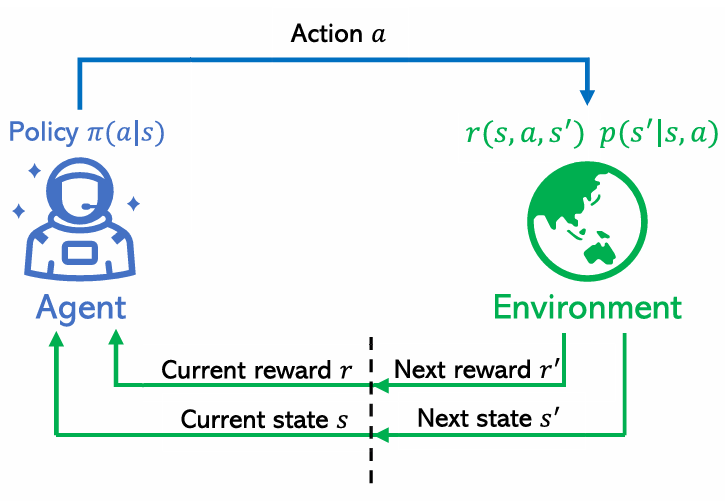
\includegraphics[width=0.5\linewidth]{Images/MDP_Diagram.png}
    \caption{Agent interaction with an MDP.}
    \label{fig:MDP_Diagram}
\end{figure}

\subsection{Reinforcement Learning}\label{sec:rl}
In RL, an agent with no prior knowledge learns to make decisions from repeated interaction with an environment, using the reward it receives as feedback \cite{LADOSZ20221}. The problem is formalised as an MDP (\cref{sec:MDP_ssSection}) \cite{LADOSZ20221, DRL_Intrusion}, and the agent learns a \emph{policy}: a probability distribution over actions $a_t$ given the state $s_t$, chosen to maximise the expected total reward. RL methods fall into two main families. \textbf{Value-based} methods learn the expected return of each action and typically choose the action with the highest estimate, while \textbf{policy-gradient} methods directly adjust the policy's parameters towards higher return \cite{williams1992reinforce}. \textbf{Actor-critic} methods combine the two: a critic learns the expected return from each state (a value function), and an actor updates the policy using the critic's estimates to judge whether an action was better or worse than expected \cite{konda1999actorcritic}. PPO and A2C are both actor-critic methods.

% =====================================================================
\section{Methodology}
\subsection{Problem Formulation}\label{sec:problem}
A cloud computing environment receives a set of jobs that must be assigned to a set of physical machines. Each job $j$ has a fixed processing duration $p_j$, a multi-dimensional vector of resource requirements $a_{jr}$ (e.g.\ CPU, memory) which it occupies for its entire duration, and a due date $d_j$ by which it should finish. Jobs are independent of one another. Each job has a priority weight $w_j$, assumed to be set externally by business needs, to reflect that some jobs matter more than others.

Jobs are served by a set of identical machines $M$, each with a fixed capacity $C_r$ for every resource $r$. A machine may process several jobs at once, provided their combined usage does not exceed its capacity in any resource. Scheduling is non-preemptive: each job is assigned to exactly one machine at a single start time $s_j$ and runs uninterrupted until completion. Time is divided into integer steps over a planning horizon $H$. The tardiness of job $j$ is
\begin{equation}\label{eq:tardiness}
    T_j = \max\left(0,\; s_j + p_j - d_j\right),
\end{equation}
and $U_j = 1$ if job $j$ finishes late ($T_j > 0$), $0$ otherwise. Notation is summarised in Appendix~\ref{sec:AppendixA} and the full constraint set in Appendix~\ref{sec:AppendixB}.

\subsection{Objective Function}\label{sec:objectives}
The first objective tried weighted the number of machines used, weighted tardiness and peak utilisation $\theta$:
\begin{equation}\label{eq:objective-v1}
    \min \; \lambda_1 \sum_{m \in M} y_m \;+\; \lambda_2 \sum_{j \in J} w_j T_j \;+\; \lambda_3\, \theta.
\end{equation}
\Cref{eq:objective-v1} could be gamed: unscheduled jobs cost nothing, so agents found high-reward schedules that left many jobs unassigned, a form of reward hacking \cite{skalse2022rewardhacking}. Its peak-utilisation term also works against energy-efficient consolidation \cite{energyaware2012, fan2007powerprovisioning}. It was replaced by a weighted sum of optional terms:
\begin{equation}\label{eq:objective-v2}
    \min \; J_{\lambda} = \underbrace{\sum_{j} w_j T_j^{2}}_{J}
          \;+\; \lambda_T \sum_{j} w_j T_j
          \;+\; \lambda_U \sum_{j} w_j U_j
          \;+\; \lambda_E E,
\end{equation}
covering squared tardiness, linear tardiness, the weighted number of late jobs (deadline violations), and energy $E$, measured as total active machine-time \cite{fan2007powerprovisioning}. The main objective of this project is $J$ alone ($\lambda_T = \lambda_U = \lambda_E = 0$). Squared tardiness penalises a few very late jobs more than many slightly late ones, whereas linear tardiness can score very different schedules equally. $J$ is evaluated over an \emph{extended horizon}: jobs are released only within $[0, H)$, but no job is ever discarded, and an unfinished job keeps accumulating tardiness until it completes. Leaving a job unscheduled is therefore always costly, which removes the loophole in \cref{eq:objective-v1}. The other terms are switched on only in the multi-objective experiments (\cref{sec:mo-method}).

\subsection{Offline and Online Cases}\label{sec:cases}
Two cases of the problem are studied. In the \textbf{offline} case all jobs are known and available at $t = 0$, and at most one job can be started per time step. In the \textbf{online} case jobs arrive (are revealed) over time according to a Poisson process \cite{kleinrock1975queueing, mao2016deeprm}, and any number of jobs may be started at the same time step.

The difficulty of the online case is set by the load factor $\rho$, which measures how busy the cluster is on average. A job $j$ brings $p_j a_{jr}$ units of work for resource $r$ (resource units multiplied by time steps). If jobs arrive at rate $\nu$ per time step, on average $\nu\,\mathbb{E}[p_j a_{jr}]$ units of work arrive per time step, while the cluster can process at most $|M|\, C_r$ units per time step. Their ratio is the standard utilisation of a queueing system \cite{kleinrock1975queueing}, and taking the largest ratio over resources picks out the bottleneck resource:
\begin{equation}\label{eq:rho}
    \rho = \max_{r \in R} \frac{\nu\, \mathbb{E}[p_j a_{jr}]}{|M|\, C_r}.
\end{equation}
For $\rho < 1$ the cluster can keep up on average; for $\rho \ge 1$ work arrives faster than it can be processed and the queue necessarily grows. For each target load, the arrival rate $\nu$ is chosen to give that $\rho$. Loads from $\rho = 0.50$ to $1.10$ are studied.

\subsection{Markov Decision Process}\label{sec:mdp}
To formulate this problem for our algorithms we use an MDP $(S, A, P, R, \gamma)$ as described in \cref{sec:MDP_ssSection}.

\paragraph{State $S$.} The state holds the features $F_j = (p_j, a_j, d_j, w_j)$ of each waiting job $j \in J_t \subseteq J$, and, for each job in the processing set $P_t \subseteq J$ (jobs that have started and not finished), $G_j = (m_j, s_j, p_j)$: its machine, start time and duration. It also holds the remaining capacity of each machine,
\begin{equation}\label{eq:remaining-capacity}
    R_{mrt} = C_r - \sum_{j \in P_t:\ m_j = m} a_{jr},
\end{equation}
and $y = (y_m)_{m \in M}$, recording which machines are switched on. This gives the state
\begin{equation}\label{eq:state}
    s_t = \big(J_t,\ P_t,\ \{F_j\}_{j \in J_t},\ \{G_j\}_{j \in P_t},\ \{R_{mrt}\}_{m \in M,\, r \in R},\ y,\ t\big).
\end{equation}
The agent also sees each machine's free capacity over the next few time steps, computed from $G_j$ (no new information, but easier to learn from).

\paragraph{Action space $A$.} At each step, the agent can assign a waiting job to a machine, or idle:
\begin{equation}\label{eq:action-flat}
    A_t = \{(j, m) : j \in J_t,\ m \in M\} \cup \{\text{idle}\}.
\end{equation}
Assignments that would exceed a machine's capacity are masked out \cite{huang2020invalidmasking}. Offline, each assignment is followed by a time step; online, the agent may make several assignments per time step, and time advances only when it idles. Idling is always allowed: deliberately leaving capacity free for later jobs is a behaviour RL could learn, and schedules that never idle can exclude the optimum \cite{giffler1960active}. An idle advances time to the next job arrival or completion, so the agent cannot idle forever.

\paragraph{Transition dynamics $P$.} An assignment $(j, m)$ moves job $j$ from $J_t$ to $P_t$ with $s_j = t$ and $m_j = m$, switching machine $m$ on if needed. When time advances, completed jobs leave the processing set by \cref{eq:processing-update} and release their capacity; online, newly arrived jobs join $J_{t+1}$. Transitions are deterministic offline, and random online only through the arrivals.
\begin{equation}\label{eq:processing-update}
    P_{t+1} = \{k \in P_t : s_k + p_k > t + 1\}.
\end{equation}

\paragraph{Reward $R$.} The reward is the negative of the objective, charged as it accrues: a late job of weight $w_j$ is charged $w_j(2k+1)$ in its $k$-th late time step, and since $\sum_{k=0}^{T_j-1}(2k+1) = T_j^2$ the charges add up to exactly $w_j T_j^2$. Maximising total reward is therefore the same as minimising $J$ in \cref{eq:objective-v2}. To give the agent earlier feedback, a potential-based shaping term is added, which provably leaves the optimal policy unchanged \cite{ng1999shaping}.

\paragraph{Action-space designs.} The full action space \cref{eq:action-flat} has 1001 actions for 100 jobs and 10 machines. Large discrete action spaces are a known difficulty for policy-gradient methods \cite{dulacarnold2015largeactionspaces}, while successful prior schedulers use far fewer actions \cite{mao2016deeprm, mao2019decima}. Six designs were therefore compared:
\begin{itemize}
    \item \textbf{Option 0 -- Direct job-machine selection.} The policy picks a (job, machine) pair from \cref{eq:action-flat}, using a pointer-network architecture \cite{vinyals2015pointernet, kool2019attention}.
    \item \textbf{Option 1 -- Rule selection.} At each decision the policy chooses which dispatching rule to apply: one of seven priority rules, each with First-Fit or Consolidate placement (\cref{sec:baselines}), making the agent a selection hyper-heuristic \cite{burke2013hyperheuristicsurvey, lassoued2026hyperheuristic}.
    \item \textbf{Option 2 -- Priority learning.} The policy picks which waiting job to start next, learning its own priority from the raw job features; the chosen job is then placed by the First-Fit rule. This is a hybrid of RL and a dispatching heuristic: RL learns the ordering, a fixed rule does the placement \cite{mao2016deeprm, min2022atctuning}.
    \item \textbf{Option 3 -- Priority learning with an ATC feature.} Option 2 with the Apparent Tardiness Cost index \cite{vepsalainen1987atc} added as an extra job feature. Option 3w is the same, restricted to the 20 most urgent jobs \cite{mao2016deeprm}.
    \item \textbf{Option 4 -- Action branching.} The job and the machine are chosen by two separate network heads instead of one joint action \cite{tavakoli2018actionbranching}.
\end{itemize}

\subsection{Learning Algorithms}\label{sec:algorithms}
All RL agents use PPO \cite{schulman2017ppo} or A2C \cite{mnih2016a3c}, as implemented in Stable-Baselines3 \cite{raffin2021sb3}. Both are actor-critic methods (\cref{sec:rl}). PPO limits how far the policy can change in a single update, which makes training more stable; A2C uses simpler, more frequent updates. Both are widely used and comparable within one framework \cite{huang2022a2cppo}.

\paragraph{Approaches tried before the final setup.} The final setup was reached through several rounds of training, diagnosis and revision. Alternatives tried along the way included reward-constrained policy optimisation (RCPO) \cite{tessler2019rcpo} and PPO-Lagrangian \cite{stooke2020pidlagrangian}, which treat tardiness as a constraint rather than a cost, dense and shaped tardiness rewards, curriculum learning, and a version in which idling was forbidden whenever a job could be placed. Under the original objective (\cref{eq:objective-v1}), none of these produced an agent that beat the best heuristic on tardiness. The final version fixed two faults in the previous one: the critic never learned, because squared-tardiness rewards are very large, and a deterministic policy could idle forever. These were fixed by reward scaling \cite{engstrom2020implementation, andrychowicz2021onpolicy}, event-driven idling (\cref{sec:mdp}) and a two-stage evaluation rule (\cref{sec:evaluation}). In addition, the critic (but not the policy) sees a summary of jobs that have not arrived yet, which reduces noise in online training without biasing the policy \cite{mao2019variance, pinto2018asymmetric}. Appendix~\ref{sec:AppendixD} gives the diagnosis.

\subsection{Methods Compared}\label{sec:baselines}
\paragraph{Dispatching heuristics.} Each heuristic combines a priority rule, which chooses the next job, with a placement rule, which chooses its machine \cite{pinedo2016scheduling}.
\begin{itemize}
    \item \textbf{Priority rules:} Earliest Deadline First (EDF) and Least Slack Time (LST), which prioritise urgency \cite{pinedo2016scheduling}; Shortest and Longest Processing Time (SPT, LPT) \cite{pinedo2016scheduling, graham1969lpt}; Weighted SPT (WSPT) \cite{smith1956wspt}; First-Come-First-Served (FCFS, also known as First-In-First-Out, FIFO); Apparent Tardiness Cost (ATC), which balances job weight, length and urgency \cite{vepsalainen1987atc}; and the weighted-tardiness rules WMDD \cite{kanet2004wmdd} and COVERT \cite{carroll1965covert}. Because the published weighted rules performed poorly under squared tardiness, three weighted variants were constructed for this project: weighted LST (WLST) and weighted EDF (WEDF), which scale a job's slack by its weight, and Marginal Delay Cost (MDC), which applies Smith's ratio rule \cite{smith1956wspt} to the marginal increase in squared tardiness. These were added after the first RL results were seen.
    \item \textbf{Placement rules:} First-Fit, Best-Fit and Worst-Fit \cite{johnson1973binpacking}, and Consolidate, an energy-aware rule that prefers machines that are already on \cite{energyaware2012}.
    \item \textbf{Tetris:} a multi-resource packing heuristic that scores job-machine pairs jointly \cite{grandl2014tetris}.
\end{itemize}

In total, the twelve priority rules and four placement rules give 48 heuristics, plus Tetris; random rule choice is included as a sanity check.

\paragraph{Metaheuristic.} Particle Swarm Optimisation (PSO) \cite{kennedy1995pso}, in which each particle encodes a job ordering that a placement rule decodes into a schedule, was evaluated in earlier rounds of the project. It was worse than the best dispatching rule in every setting tested, so it is not part of the final comparison.

\paragraph{Exact solver.} CP-SAT \cite{ortools}, a constraint-programming solver, models the problem of Appendix~\ref{sec:AppendixB} exactly. Within a time limit it returns the best schedule it has found, whose $J$ is an upper bound on the optimum, together with a proven lower bound on the optimum. When the two meet, the schedule is proven optimal. CP-SAT was given 60 seconds per instance.

\subsection{Implementation}\label{sec:implementation}
The environment, agents and evaluation pipeline are implemented in Python\footnote{\url{https://github.com/Ethan-Ty-Riekert/Neural-Knapsack-Research-Project}} using Gymnasium and Stable-Baselines3 \cite{raffin2021sb3}. The environment and the translation of the mathematical formulation into code were written by hand; model implementation, training and evaluation were done with the help of Claude Code (see the Generative AI Use Statement).

\subsection{Experimental Setup}\label{sec:setup}
\paragraph{Instances.} Offline instances have 100 jobs, 10 machines and 4 resources with $C_r = 30$, and $H = 100$. Job durations and resource demands are drawn uniformly from $\{1, \dots, 9\}$, and weights from $\{1, \dots, 5\}$. Deadline tightness is set by the tardiness factor TF \cite{potts1985wtardiness}: larger TF means tighter deadlines on average. The main setting uses TF $= 0.5$ (medium), with 0.2 and 0.8 as loose and tight variants. A unit-weight setting ($w_j = 1$) isolates the effect of job weights. Online instances add Poisson arrivals at loads $\rho \in \{0.50, 0.75, 0.95, 1.10\}$; each job's deadline is its arrival time plus a random slack, the online counterpart of TF. Online job sizes are log-normal (right-skewed, like real cluster traces \cite{reiss2012googletrace, cortez2017resourcecentral}). Agents were trained on TF $= 0.5$ offline and $\rho = 0.95$ online. Appendix~\ref{sec:AppendixD} gives the exact distributions.

\paragraph{Training and tuning.} An agent learns over episodes, each a complete, newly generated problem instance, so it never trains on the same problem twice. Training, validation (20 instances) and test (50 instances) use disjoint random seeds, so test instances are never seen in training or tuning. Every combination of design (6), algorithm (2) and case (2) had its own hyperparameter search, 24 studies in all, run with the same protocol: Optuna \cite{akiba2019optuna} with the TPE sampler \cite{bergstra2011tpe}, 12 trials of 300,000 steps, the first trial always being the library defaults. Poor trials were stopped early by median pruning, which compares a trial's validation $J$ with the median of earlier trials \emph{at the same training step}. Each study keeps one best configuration, chosen on the 20 validation instances. That configuration was then retrained with 3 random seeds for 1,000,000 steps offline and 300,000 steps online, and results are the mean and standard deviation over the seeds. A follow-up trained online Options 0, 2 and 3 (PPO) for 1,000,000 steps, and Option 2 for 2,000,000. Appendices~\ref{sec:AppendixC} and~\ref{sec:AppendixD} list the search space and protocol details.

\paragraph{Evaluation.}\label{sec:evaluation} Every method, RL and baseline, is evaluated on the same 50 held-out test instances for each setting. RL agents act deterministically using a two-stage rule: idle if the probability of idling is at least the total probability of all job actions, otherwise take the most likely job action. A plain ``most likely action'' rule is biased towards idling (\cref{sec:algorithms}). We report mean $J$ over the test instances; for RL this is averaged over the 3 seeds, with the standard deviation across seeds. The heuristics are deterministic, so they were run once; their standard deviation is across instances.

We also record metrics that were not optimised, such as the on-time rate, number of late jobs, maximum tardiness and energy. Any pattern in these is a side effect of optimising $J$ rather than a learned trade-off, so it is interpreted with caution. Some metrics are uninformative by construction: offline, exactly one job starts per time step, so the mean waiting time is 49.5 for every method.

\paragraph{Multi-objective experiments.}\label{sec:mo-method} To test whether RL's relative performance depends on the objective, every method was also scored on composite objectives $J_\lambda$ (\cref{eq:objective-v2}). The weights $\lambda_T, \lambda_U, \lambda_E$ are set separately for each setting, so that each added term equals $J$ on the best heuristic's schedule; this prevents any term from dominating merely because of its units. Each weight is then multiplied by 0.25, 0.5, 1, 2 and 4. In addition to the agents trained on $J$ alone, Option 2 and 3 PPO agents were trained directly on several composite objectives (300,000 steps offline with default hyperparameters, 3 seeds; 1,000,000 steps online).

% =====================================================================
\section{Results}\label{sec:results}
All results below are on the 50 held-out test instances; lower $J$ is better. Full tables for every setting and metric are on the project's GitHub \href{https://github.com/Ethan-Ty-Riekert/Neural-Knapsack-Research-Project/tree/main/Results}{results page}.

\subsection{RL against heuristics on the main objective}\label{sec:res-main}
\Cref{tab:main} and \cref{fig:offline} summarise the main comparison. Offline, with weighted jobs, the best RL agent (Option 2, PPO) reaches $J = 28{,}061$, 5.2\% above the best heuristic, WLST ($26{,}670$). RL's standard deviation across seeds is small (219), so the gap is not an artefact of one unlucky seed. Every design except Option 1 lands within 12\% of WLST, and all of them beat every published rule: the best of these, LST, scores $39{,}536$, 29\% worse than the best RL agent. The weighted rules WLST, WEDF and MDC were designed for this project after RL had beaten LST, and only WLST beats RL. CP-SAT's best schedule after 60 seconds ($35{,}681$) is worse than both RL and WLST, so it gives no useful bound on how far either is from optimal at this size. On 15-job instances, however, CP-SAT proved 13 of 15 instances optimal, and LST matched the optimum on every one.

When every job has the same weight, the problem is easier for the heuristics: LST scores $13{,}098$, and the best RL agents either reproduce it exactly (Option 1) or come within 0.8\% (Option 2).

Online at $\rho = 0.95$, under the standard protocol (300,000 steps), every RL design is far behind the best heuristic, EDF+Consolidate ($21{,}986$): the best is Option 1 A2C at $37{,}812$ (+72\%). The online gap is mainly a training-budget problem (\cref{sec:res-online}).

\begin{table}[htbp]
\centering
\caption{Mean $J$ on 50 test instances (lower is better). RL: mean $\pm$ standard deviation over 3 seeds, best algorithm per design; heuristics are deterministic. Online RL is shown at the standard 300k-step budget; longer budgets are in \cref{tab:budget}.}
\label{tab:main}
\begin{tabular}{lrrr}
\toprule
Method & Offline, weighted & Offline, $w_j = 1$ & Online, $\rho = 0.95$ \\
\midrule
Best heuristic & 26,670 (WLST) & 13,098 (LST) & 21,986 (EDF+Cons.) \\
LST+FirstFit & 39,536 & 13,098 & 38,831 \\
EDF+FirstFit & 41,302 & 13,757 & 40,381 \\
CP-SAT (60 s) & 35,681 & 16,469 & -- \\
\midrule
Option 0 (job--machine pairs) & 29,696 $\pm$ 833 & 13,494 $\pm$ 276 & 44,920 $\pm$ 0 \\
Option 1 (rule selection) & 38,645 $\pm$ 142 & 13,098 $\pm$ 0 & 37,812 $\pm$ 8,893 \\
Option 2 (priority) & \textbf{28,061 $\pm$ 219} & 13,207 $\pm$ 28 & 39,947 $\pm$ 11,949 \\
Option 3 (priority + ATC) & 28,282 $\pm$ 537 & 13,496 $\pm$ 98 & 44,827 $\pm$ 2,890 \\
Option 4 (action branching) & 28,577 $\pm$ 43 & 13,411 $\pm$ 181 & 139,721 $\pm$ 101,396 \\
\midrule
Best RL vs best heuristic & +5.2\% & 0.0\% & +72\% \\
\bottomrule
\end{tabular}
\end{table}
% NOTE (Ty): Option 3w is left out to keep the table small (offline 28,695 +/- 1,133; online 56,493 +/- 11,019).

\begin{figure}[htbp]
\centering
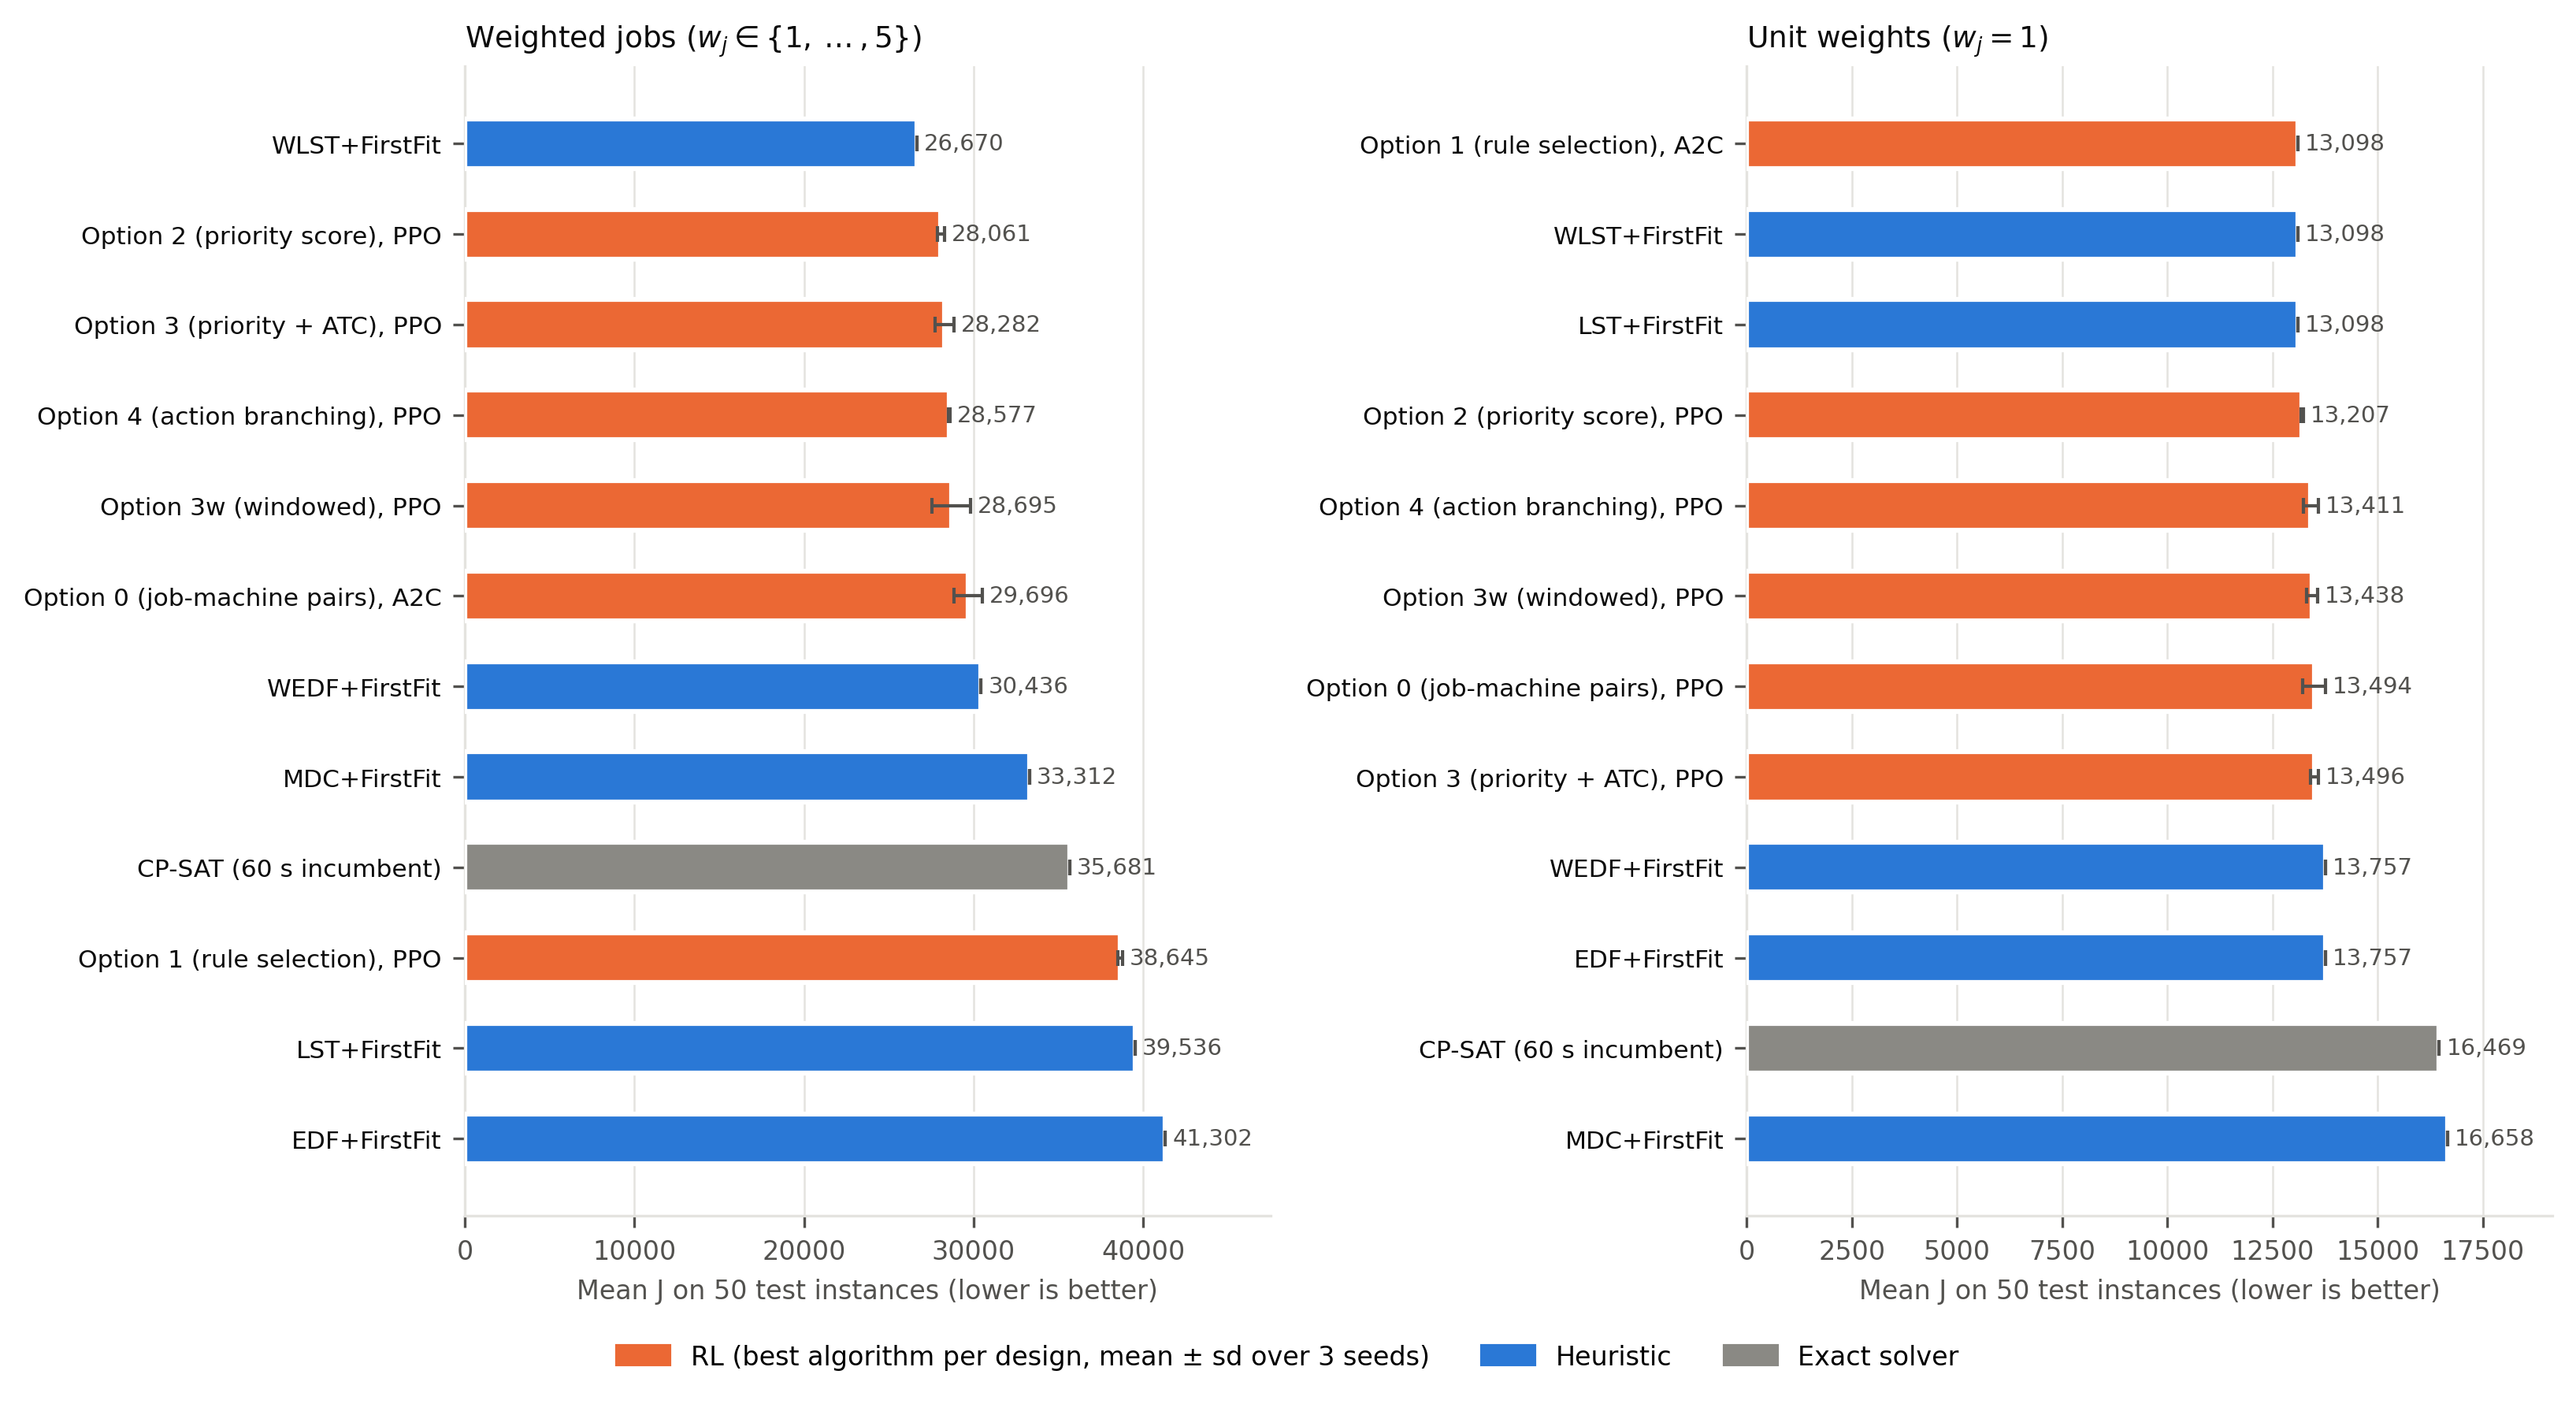
\includegraphics[width=\linewidth]{Images/v2_offline_designs.png}
\caption{Offline results: the best final agent of each design (orange, mean $\pm$ s.d.\ over 3 seeds) against the leading heuristics (blue) and CP-SAT's 60-second schedule (grey). Left: weighted jobs; right: unit weights.}
\label{fig:offline}
\end{figure}

\subsection{Combined objectives}\label{sec:res-mo}
When the objective rewards more than squared tardiness, RL overtakes the best heuristic offline (\cref{fig:mo}, \cref{tab:mo}). Once linear tardiness is weighted at least as heavily as the reference ($\times 1$), the best RL agent beats the best heuristic by 1.8--10.3\%; with late jobs added at weights $\times 0.5$ to $\times 4$, by 1.4--10.0\%; and with all four terms, by 8.6\%. The advantage grows with the weight of the added term up to $\times 2$--$\times 4$. At moderate weights, the winning agents were trained on $J$ alone; at the largest weights, agents trained on the composite objective win.

This advantage depends on job weights and on the setting. With unit weights, RL never beats LST on any composite objective (0.0\% to +10.8\%). Online, the best RL agent stays within 0.1--6.5\% of the best heuristic on every composite but never beats it, and that agent is a single seed.

\begin{table}[htbp]
\centering
\caption{Best RL agent against the best heuristic on composite objectives, offline with weighted jobs. Negative means RL is better. Weights are multiples of the reference values ($\lambda_T = 15.8$, $\lambda_U = 146$, $\lambda_E = 153$).}
\label{tab:mo}
\begin{tabular}{lrrr}
\toprule
Objective & Best heuristic & Best RL & RL vs heuristic \\
\midrule
$J$ only & 26,670 & 28,061 & +5.2\% \\
$J$ + linear tardiness ($\times 1$) & 53,300 & 52,363 & $-1.8$\% \\
$J$ + linear tardiness ($\times 4$) & 133,190 & 119,419 & $-10.3$\% \\
$J$ + late jobs ($\times 1$) & 53,421 & 48,101 & $-10.0$\% \\
$J$ + late jobs ($\times 4$) & 88,835 & 87,569 & $-1.4$\% \\
$J$ + energy ($\times 1$) & 52,274 & 54,398 & +4.1\% \\
All four terms ($\times 1$) & 105,654 & 96,541 & $-8.6$\% \\
\bottomrule
\end{tabular}
\end{table}

\begin{figure}[htbp]
\centering
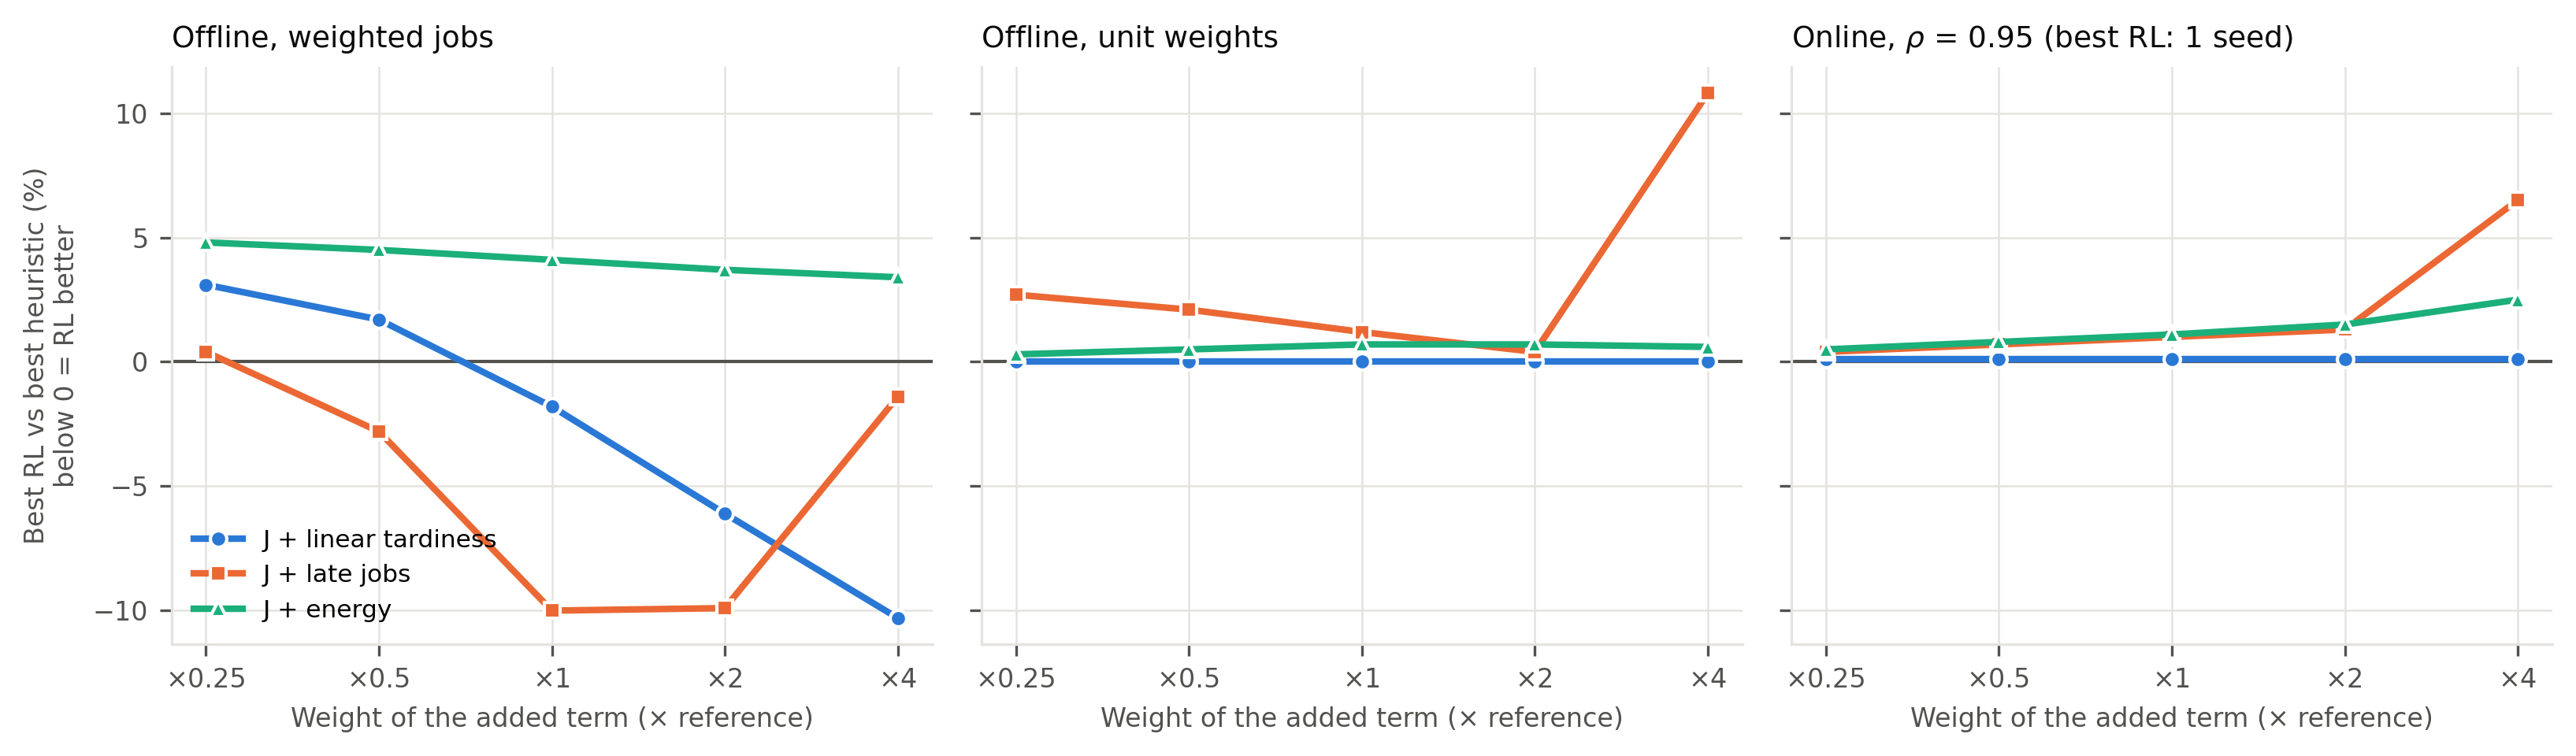
\includegraphics[width=\linewidth]{Images/v2_multiobjective_gap.png}
\caption{Best RL agent relative to the best heuristic as the weight of each added term grows (below zero: RL better). Left: offline, weighted jobs; middle: offline, unit weights (RL agents trained on $J$ only); right: online, $\rho = 0.95$ (best RL agent is a single seed).}
\label{fig:mo}
\end{figure}

\subsection{Online training budget}\label{sec:res-online}
More training closes most of the online gap for Option 2 but not for Option 0 (\cref{tab:budget}, \cref{fig:budget}). Option 2's mean $J$ falls from $39{,}947$ at 300k steps to $26{,}515$ at 1M (+21\% over EDF+Consolidate) and $24{,}921$ at 2M (+13\%, 2 seeds), and its best 1M seed is within 4.3\% of the heuristic. Option 0 improves on average but remains 55\% behind at 1M. The single best online run, an Option 2 agent trained for 1M steps on $J$ plus linear tardiness, matched EDF+Consolidate ($22{,}000$ vs $21{,}986$, +0.1\%), but this is one seed. Online A2C did not learn: Option 0 A2C produced the same schedule as FCFS+FirstFit ($J = 44{,}920$) on all three seeds.

\begin{table}[htbp]
\centering
\caption{Online ($\rho = 0.95$) mean test $J$ by training budget, PPO, mean $\pm$ s.d.\ over seeds (EDF+Consolidate: 21,986).}
\label{tab:budget}
\begin{tabular}{lrrr}
\toprule
Design & 300k steps & 1M steps & 2M steps \\
\midrule
Option 0 & 49,404 $\pm$ 18,050 & 33,966 $\pm$ 3,699 & -- \\
Option 2 & 39,947 $\pm$ 11,949 & 26,515 $\pm$ 4,564 & 24,921 $\pm$ 2,555 (2 seeds) \\
Option 3 & 44,827 $\pm$ 2,890 & 30,611 $\pm$ 1,909 & -- \\
\bottomrule
\end{tabular}
\end{table}

\begin{figure}[htbp]
\centering
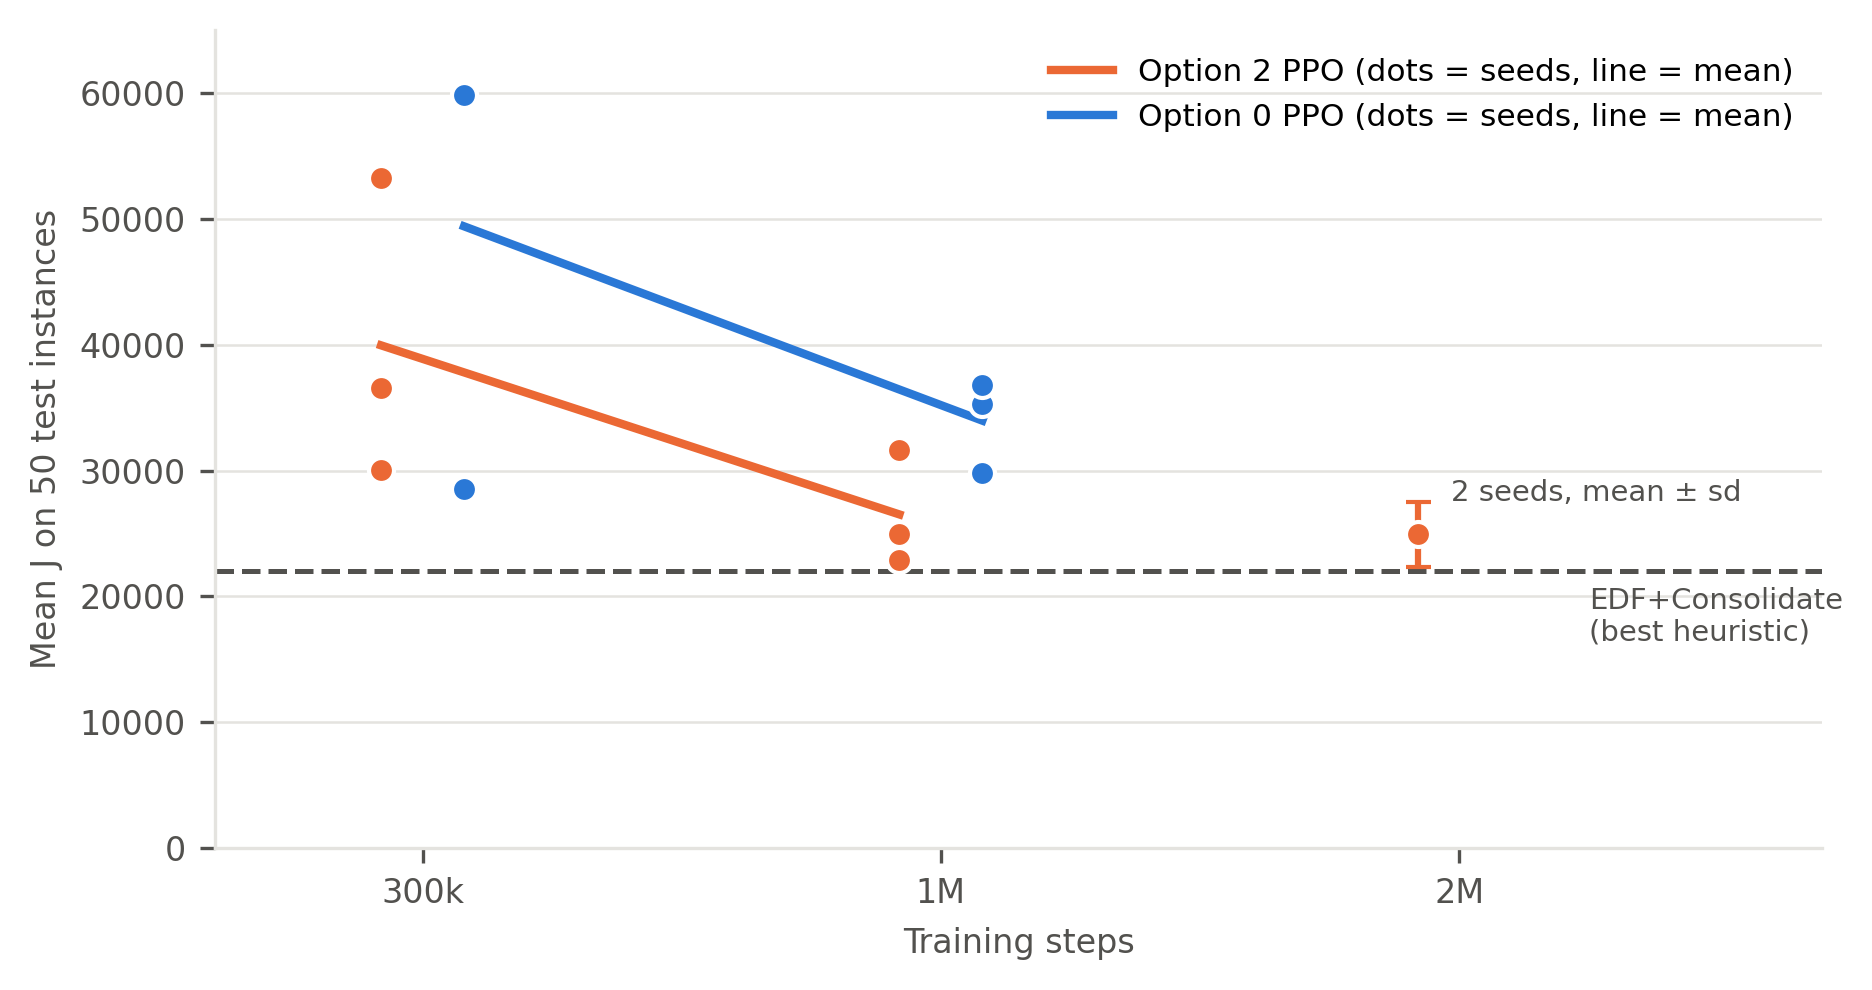
\includegraphics[width=0.75\linewidth]{Images/v2_online_budget.png}
\caption{Online test $J$ of PPO Options 0 and 2 by training budget; dots are individual seeds. The dashed line is the best heuristic.}
\label{fig:budget}
\end{figure}

\subsection{Other findings}\label{sec:res-other}
\paragraph{Action-space design.} Learning a job priority (Options 2 and 3) worked best in every setting. Picking job-machine pairs directly (Option 0) was 6\% worse offline and still 55\% behind online after 1M steps, and choosing job and machine with two heads (Option 4), competitive offline, failed online ($J = 139{,}721$). Rule selection (Option 1) mostly collapsed onto a single rule: with unit weights it reproduced LST exactly on all three seeds, and with weighted jobs its schedules had the same number of late jobs as LST (61.0) and a similar $J$ (within 2.3\% of LST).

\paragraph{Training stability.} In 8 independent offline runs of the same Option 2 configuration (default hyperparameters, 300k steps), one diverged ($J = 69{,}367$ against $28{,}352$--$30{,}925$ for the other seven). Online seeds differ much more: Option 2 at 300k steps ranged from $30{,}076$ to $53{,}231$.

\paragraph{Energy.} RL lost to the best heuristic (WLST+Consolidate) on every $J$ + energy objective, by 3.4--4.8\%. Training with the energy term made no run diverge in 8 seeds, but it did not make training meaningfully more stable either: those runs were 5--25\% worse on $J$, the expected cost of trading $J$ for energy.

\paragraph{No single heuristic wins everywhere.} The best rule changed with deadline tightness and load: EDF with loose offline deadlines (TF $= 0.2$, where it reaches $J = 0$), WLST with medium and tight deadlines, LST with unit weights, WLST+Consolidate online at $\rho = 0.50$ and $0.75$, EDF+Consolidate at $\rho = 0.95$, and MDC+Consolidate under overload ($\rho = 1.10$). Online, Consolidate placement was best at every load.

\paragraph{Hyperparameter tuning.} The library defaults were the best configuration in 8 of the 24 studies, including both studies for Options 0 and 2 PPO online that were stopped early.

% =====================================================================
\section{Discussion}\label{sec:discussion}
\paragraph{When does RL beat the heuristics?} Our results suggest three conditions. First, \emph{the objective must not be one that a simple rule already solves well}. With unit weights and squared tardiness, LST matched every proven optimum on small instances, and RL could at best reproduce it. When the objective mixes several goals (\cref{sec:res-mo}), no single rule is designed for the combination, and RL won by up to 10\%. Second, \emph{jobs must differ in importance}. The offline multi-objective advantage disappeared with unit weights. Weights give a learned priority more to work with, since the right order now depends jointly on deadline, length and weight. Third, \emph{the agent must be trained enough for the setting}. Offline, 1M steps was enough to come within 5\% of the best heuristic. Online, 300k steps left RL 70\% behind, and 1--2M steps closed most of the gap for the best design.

\paragraph{RL and heuristic design.} The best offline heuristic, WLST, did not exist at the start of the project: it was constructed after RL agents had beaten every published rule by 29\%. One reading is that RL lost to WLST. A fairer reading is that RL found, automatically and within 5\%, a level of performance that took a purpose-built rule to match. This suggests that RL could also serve as a tool for heuristic design, by revealing that better rules exist for a new objective. It also shows how much results depend on the choice of baselines. Studies that compare RL only with standard rules would have reported a clear RL win here.

\paragraph{Why the multi-objective gains need care.} At moderate weights, the agents that won the composite objectives were trained on $J$ alone. Their schedules happened to have fewer late jobs and lower linear tardiness than WLST's (for example, Option 0 A2C: 52.7 late jobs against 61.7). WLST is tuned for squared tardiness and gives up the other metrics to get it. This part of the advantage is therefore a side effect of how RL schedules, not a trade-off it learned, and it is exactly the kind of pattern in non-optimised metrics that must not be over-interpreted. At larger weights, agents trained on the composite objective took over, which does indicate learning. Re-running these agents with the tuned settings and full 1M-step budget is in progress.

\paragraph{Why online is harder.} Online returns depend heavily on the random arrival sequence, which the agent cannot predict, so the training signal is much noisier than offline \cite{mao2019variance}. Online episodes are also roughly ten times longer, and the observation has to cover over a thousand job slots. Both effects mean more samples are needed, consistent with the budget results. Option 0's much larger action space compounds the problem \cite{dulacarnold2015largeactionspaces}.

\paragraph{Action spaces and energy.} Priority learning worked best, in line with DeepRM and Decima, which also let the network choose the job and leave placement to the system \cite{mao2016deeprm, mao2019decima}. Rule selection collapsed onto one rule, so it can at best match the best rule in its menu. Options 2 and 3 always place with First-Fit and so cannot consolidate jobs onto fewer machines, a likely (still untested) reason they lose on energy.

\paragraph{Practical considerations.} RL training is unstable (one diverged run in eight) and expensive, and tuning helped little: the defaults were best in 8 of 24 studies, consistent with the known sensitivity of RL to hyperparameters and the small tuning budgets typically used \cite{eimer2023hyperparams}. A heuristic needs no training and behaves the same every time. RL is therefore worth its cost mainly where the objective is complex and weighted, and where enough compute is available.

\paragraph{Limitations.} All instances are synthetic and of one size (100 jobs, 10 machines), and results use 3 seeds. Picking the best of many RL variants on the test set slightly favours RL, although the best heuristic is picked the same way. CP-SAT did not reach optimality at 100 jobs, so the distance of RL and WLST from the optimum is unknown. The online multi-objective and 2M-step results rest on one and two seeds, and three online studies were stopped early.

% =====================================================================
\section{Conclusion}\label{sec:conclusion}
This project formulated cloud resource allocation as a multi-resource scheduling problem and an MDP, built an offline and online simulation environment, and compared six RL action-space designs, trained with PPO and A2C under one uniform protocol, against 49 heuristics and an exact solver. On the main objective, weighted squared tardiness, RL came within 5\% of the best heuristic offline and beat every published rule by 29\%, but did not beat the best rule, which was purpose-built for that objective. RL did beat the best heuristic, by 2--10\%, once linear tardiness or late jobs were added to the objective, provided jobs had different weights. Online, RL needed several times more training to approach the heuristics, and it never won when energy was part of the objective. Learning a job priority was the most effective design. Getting RL to train reliably required careful diagnosis: reward scaling and event-driven idling were essential. In short, RL is most competitive when the objective combines goals that no single rule targets, jobs differ in importance, and training is sufficient. Where a simple rule is already near-optimal, the heuristic remains the better choice.

\section{Future Work}
\begin{itemize}
    \item Extend the online study with longer training and more seeds, since the online gap was mainly a training-budget problem.
    \item Test generalisation to other deadline tightness and loads (in progress), larger clusters, and real traces such as Google's \cite{reiss2012googletrace} or Azure's \cite{cortez2017resourcecentral}.
    \item Let RL choose placement as well as job order, e.g.\ with a consolidating placement rule, to address the energy gap.
    \item Train one agent conditioned on the objective weights \cite{abels2019dynamicweights, hayes2022morlguide}, and try graph neural network encoders \cite{gnn2024jsspsurvey}.
    \item Use RL for heuristic discovery: extract interpretable rules from learned priorities.
\end{itemize}

% =====================================================================
\section*{Data Management Plan}
All code, raw results (per-instance metrics for every method and seed), processed tables and figures, Optuna study logs and the chronological experiment log are in the public GitHub repository\footnote{\url{https://github.com/Ethan-Ty-Riekert/Neural-Knapsack-Research-Project}}. Results are under \texttt{Results/} (raw runs, tuning studies, and the processed \texttt{ALL\_RESULTS} archive), and every number in this report can be regenerated from them with the scripts provided. All instances are synthetic and generated from fixed random seeds, so no personal or sensitive data is involved. Trained model files are regenerated by the training scripts and are not version-controlled. The version cited in this report is a tagged release on the \texttt{main} branch.

\section*{Generative AI Use Statement}
Claude Code (Anthropic) was used as a coding and research assistant. The original environment and the translation of the mathematical formulation into code were done by hand. Claude Code was used to implement models, training and evaluation, and to run experiments, under the following rules:
\begin{itemize}
    \item \textbf{Context.} Claude was given the latest version of the report, formulations and experiment logs.
    \item \textbf{Rules.} Every design decision had to be cited and justified, or derived, and implementation and discussion had to remain mathematically grounded.
    \item \textbf{Benchmarking and results.} Experiments were run by Claude from a queue, and every result was reviewed personally.
    \item \textbf{Diagnostics and research.} Unexpected results and failures were investigated and checked against the literature.
    \item \textbf{Recording.} Every decision and result was recorded in an experiment log.
\end{itemize}
All modelling decisions and formulations were reviewed and approved personally. Using Claude allowed far more experiments, analyses and model iterations than would otherwise have been possible, and made it easier to discuss modelling decisions against other papers. Separate Claude agents were also used weekly to check the code's efficiency, mathematical rigour and factual accuracy. Claude was also used to help edit the text of this report; all content was reviewed and approved by the author.

\newpage
\bibliographystyle{IEEEtran}
\bibliography{references}

\newpage
\appendix
\section{Nomenclature}\label{sec:AppendixA}
\begin{table}[htbp]
\centering
\caption{Nomenclature}
\label{tab:nomenclature}
\begin{tabular}{ll}
\toprule
\multicolumn{2}{l}{\textbf{Sets}}\\
\midrule
$J$ & Set of jobs, indexed by $j$ \\
$J_t$ & Jobs waiting (arrived, not yet started) at time $t$ \\
$P_t$ & Jobs processing (started, not finished) at time $t$ \\
$M$ & Set of machines, indexed by $m$ \\
$R$ & Set of resource types, indexed by $r$ \\
$\mathcal{T}$ & Set of discrete time periods, indexed by $t$ \\
\midrule
\multicolumn{2}{l}{\textbf{Parameters}}\\
\midrule
$p_j$ & Processing duration of job $j$ \\
$a_{jr}$ & Requirement of job $j$ for resource $r$ \\
$C_r$ & Capacity of each machine for resource $r$ \\
$H$ & Length of the planning horizon \\
$d_j$ & Due date of job $j$ \\
$w_j$ & Priority weight of job $j$ \\
$\tau_j$ & Arrival time of job $j$ ($0$ offline) \\
$\nu$, $\rho$ & Arrival rate and load factor (online) \\
TF, RDD & Tardiness factor and due-date range (offline deadlines) \\
$\lambda_1, \lambda_2, \lambda_3$ & Weights in the initial objective \cref{eq:objective-v1} \\
$\lambda_T, \lambda_U, \lambda_E$ & Weights in the final objective \cref{eq:objective-v2} \\
\midrule
\multicolumn{2}{l}{\textbf{Decision variables}}\\
\midrule
$x_{jmt}$ & 1 if job $j$ starts on machine $m$ at time $t$; 0 otherwise \\
$y_m$ & 1 if machine $m$ is used; 0 otherwise \\
$s_j$ & Start time of job $j$ \\
$T_j$ & Tardiness of job $j$, $\max(0, s_j + p_j - d_j)$ \\
$U_j$ & 1 if job $j$ finishes after $d_j$; 0 otherwise \\
$E$ & Energy: total active machine-time \\
$U_{mrt}$ & Total usage of resource $r$ on machine $m$ at time $t$ \\
$\theta$ & Peak utilisation ratio, $\max_{m,r,t} U_{mrt}/C_r$ \\
\bottomrule
\end{tabular}
\end{table}

\section{Constraints}\label{sec:AppendixB}
Let $\mathcal{T} = \{0, 1, \dots, \bar{H}\}$, where $\bar{H}$ is any upper bound on the time to finish all jobs (e.g.\ $H + \sum_j p_j$, under the extended horizon). For each job, let $\mathcal{T}_j = \{t \in \mathcal{T} : \tau_j \le t \le \bar{H} - p_j\}$ be its feasible start times.

\paragraph{Assignment.} Each job starts exactly once, on exactly one machine, and never before it arrives:
\begin{equation}\label{con:assign}
    \sum_{m \in M} \sum_{t \in \mathcal{T}_j} x_{jmt} = 1, \qquad \forall j \in J.
\end{equation}
\paragraph{Offline start rate.} Offline, at most one job starts per time step:
\begin{equation}\label{con:one-start}
    \sum_{j \in J} \sum_{m \in M} x_{jmt} \le 1, \qquad \forall t \in \mathcal{T}.
\end{equation}
\paragraph{Machine activation.} A job can only be placed on an active machine:
\begin{equation}\label{con:machine-use}
    x_{jmt} \le y_m, \qquad \forall j \in J,\ m \in M,\ t \in \mathcal{T}_j.
\end{equation}
\paragraph{Start time.}
\begin{equation}\label{con:start-time}
    s_j = \sum_{m \in M} \sum_{t \in \mathcal{T}_j} t\, x_{jmt}, \qquad \forall j \in J.
\end{equation}
\paragraph{Resource usage and capacity.} A job started at $t'$ occupies its resources during $[t', t'+p_j)$, so the usage at time $t$ counts every job started within the previous $p_j$ steps. Usage may never exceed capacity:
\begin{equation}\label{con:resource-usage}
    U_{mrt} = \sum_{j \in J} \; \sum_{\substack{t' \in \mathcal{T}_j \\ t - p_j < t' \le t}} a_{jr}\, x_{jmt'} \;\le\; C_r, \qquad \forall m \in M,\ r \in R,\ t \in \mathcal{T}.
\end{equation}
\paragraph{Tardiness, late jobs and peak utilisation.}
\begin{equation}\label{con:tardiness}
    T_j \ge s_j + p_j - d_j, \quad T_j \ge 0, \quad T_j \le \bar{H}\, U_j, \qquad \forall j \in J,
\end{equation}
\begin{equation}\label{con:theta}
    \theta \ge \frac{U_{mrt}}{C_r}, \qquad \forall m \in M,\ r \in R,\ t \in \mathcal{T}.
\end{equation}
Because the objectives are minimised and increase with $T_j$, $U_j$ and $\theta$, these inequalities hold with equality at the optimum. Finally, $x_{jmt}, y_m, U_j \in \{0, 1\}$.

\section{Hyperparameter Search Space}\label{sec:AppendixC}
\begin{table}[htbp]
\centering
\caption{Hyperparameters searched by Optuna (ranges after \cite{andrychowicz2021onpolicy}). ``log'' means sampled log-uniformly; lists are categorical choices. Trial 0 of every study used the library defaults instead.}
\label{tab:hp}
\begin{tabular}{lll}
\toprule
Hyperparameter & PPO & A2C \\
\midrule
Learning rate & $3\times10^{-5}$ -- $10^{-3}$ (log) & $10^{-4}$ -- $3\times10^{-3}$ (log) \\
Rollout length (all 4 environments) & 2048, 4096, 8192, 16384 & 20, 80, 320 \\
Minibatch size & 64, 256, 1024 & -- \\
Epochs per update & 3, 5, 10 & -- \\
Discount factor $\gamma$ & 0.99, 0.995, 0.999 & 0.99, 0.995, 0.999 \\
GAE $\lambda$ & 0.9, 0.95, 0.98 & 0.9, 0.95, 1.0 \\
Clip range & 0.1, 0.2, 0.3 & -- \\
Entropy coefficient & $10^{-4}$ -- $3\times10^{-2}$ (log) & $10^{-4}$ -- $3\times10^{-2}$ (log) \\
\bottomrule
\end{tabular}
\end{table}

\section{Experimental Details}\label{sec:AppendixD}
\paragraph{Offline deadlines.} Following Potts and Van Wassenhove \cite{potts1985wtardiness}, each $d_j$ is drawn uniformly from $[\,\bar{C}(1 - \mathrm{TF} - \mathrm{RDD}/2),\ \bar{C}(1 - \mathrm{TF} + \mathrm{RDD}/2)\,]$ and is at least $p_j$. Here $\bar{C}$ is a lower bound on the time to finish all jobs (the larger of the number of jobs, since one job starts per step, and the total work divided by the cluster's capacity), TF is the tardiness factor and RDD $= 0.6$ the range of due dates, which sets how spread out deadlines are.

\paragraph{Online deadlines and job sizes.} A job's deadline is its arrival time plus a slack drawn uniformly from $\{10, \dots, 60\}$ time steps ($\{5, \dots, 25\}$ in a tight-deadline variant). Durations and demands are log-normal, not Gaussian: the logarithm of the size is normally distributed (with $\sigma = 1$), giving many small jobs and a few large ones. The location parameter is set so that the mean equals that of the offline uniform distribution, and sizes are capped at four times the offline maximum (durations of at most 40 steps).

\paragraph{Tuning protocol.} Each of the 24 studies ran 12 trials of 300,000 steps with 4 parallel environments; trial 0 used the Stable-Baselines3 defaults, which lie outside the log-scaled search space (the default entropy coefficient is 0). Every 75,000 steps, a trial reported its mean $J$ on 5 validation instances. Optuna's median pruner stopped the trial if this was worse than the median of the values earlier trials had reported at the same step; pruning only starts after 5 trials have finished. A completed trial's score is its mean $J$ on all 20 validation instances, and the best score gives the study's single chosen configuration. The offline configuration was reused for the unit-weight setting. Three online PPO studies (Options 0, 2 and 4) trained at about 20 steps per second, roughly 4--5 hours per trial, and were stopped after 3--7 trials to meet the project deadline; the best completed trial was used as usual. The defaults were the best configuration in 8 of the 24 studies.

\paragraph{Faults fixed in the final training version.} Each fault was measured directly in training logs.
\begin{enumerate}[nosep]
    \item \emph{The critic did not learn.} Squared-tardiness returns are in the hundreds to thousands, and the value and policy losses share one clipped gradient, so the value error swamped each update. The critic explained none of the variance in returns, and A2C policies stayed close to uniformly random. Rewards are now divided by a running estimate of the standard deviation of the return \cite{engstrom2020implementation, andrychowicz2021onpolicy}; afterwards the critic explained 30--99.9\% of the variance.
    \item \emph{Deterministic evaluation idled.} Idle is a single action, while the probability of starting a job is split across many (job, machine) actions. For an undecided policy, idle could be the single most likely action in every state, so a ``most likely action'' rule idled indefinitely even though the trained (sampling) policy placed jobs 98\% of the time. The two-stage rule of \cref{sec:evaluation} fixes this, and is identical to the most-likely-action rule for confident policies.
    \item \emph{Idling could repeat forever.} An idle used to advance time by one step and return the agent to an unchanged decision. Event-driven idling advances to the next arrival or completion instead. Waiting between events never helps, since a job that fits at an intermediate step also fits now and finishes earlier, so no schedule is lost.
\end{enumerate}
Together, these changes reduced offline Option 0 A2C's validation $J$ from 234,116 to 43,164.

\end{document}
